\documentclass[a4paper, 12pt]{article}	 % A4 paper and 11pt font size

\usepackage[vietnamese]{babel}  % Hỗ trợ tiếng Việt
\usepackage[svgnames]{xcolor} % Sử dụng thêm màumàu
\usepackage[a4paper, left=2cm, right=2cm, top=1cm, bottom=2.5cm, footskip=1.2cm]{geometry}  % Chỉnh kích thước tài liệu

\usepackage{graphicx}
\graphicspath{ {./images/} }

\usepackage[T1]{fontenc}
\usepackage{tgschola}

\setlength\parindent{0pt} % Đặt các đoạn luôn sát lề trái

\title{\textbf{\color{DarkRed} TÀI LIỆU ĐỀ XUẤT Ý TƯỞNG}}
\author{}
\date{} % No date

%%%%%% Bắt đầu tài liệu

\begin{document}

\maketitle % In tiêu đề

% Thông tin chung
\vspace{-1cm}
\textbf{Tên đề tài:} Hệ thống danh tiếng phục vụ xác thực hồ sơ và đánh giá kỹ năng
\vspace{5pt}

\begin{tabular}{@{} l l l l @{}}
  \textbf{Sinh viên thực hiện:} & Nguyễn Hải Tuyên & -- & 21127474 \\
                                & Trần Minh Đạt    & -- & 21127570
\end{tabular}
\vspace{5pt}

\textbf{Giảng viên hướng dẫn:} PGS.TS Nguyễn Đình Thúc
\vspace{5pt}

\textbf{Bộ môn:} Công nghệ tri thức

\rule{\textwidth}{0.4pt}

\section*{Mô tả tổng quan về hệ thống}

Hệ thống danh tiếng phục vụ xác thực hồ sơ và đánh giá kỹ năng là một nền tảng dựa trên công nghệ \textbf{blockchain}, 
được thiết kế để xác minh trình độ học vấn, kỹ năng và kinh nghiệm của cá nhân trong lĩnh vực Công nghệ thông tin. 
Hệ thống giúp đảm bảo tính minh bạch, tin cậy và không thể thay đổi của dữ liệu, qua đó hỗ trợ các tổ chức, 
doanh nghiệp và cá nhân xác thực một cách chính xác năng lực của ứng viên hoặc đối tác.
Mục tiêu của hệ thống là tạo ra một môi trường đánh giá khách quan, giúp nâng cao uy tín và giá trị của 
hồ sơ cá nhân trong ngành Công nghệ thông tin.

\section*{Đối tượng sử dụng}

\textbf{- Học sinh, sinh viên và người đang đi làm:} sử dụng hệ thống để thực hiện các \textit{thử thách} (challenges) nhằm tích lũy kiến thức,
rèn luyện bản thân, cũng như nâng cao uy tín cá nhân.
\vspace{4pt}

\textbf{- Tổ chức, doanh nghiệp:} ứng dụng hệ thống để đánh giá kỹ năng, xác thực tính chính xác của hồ sơ ứng viên, 
và hỗ trợ quá trình tuyển dụng dựa trên dữ liệu minh bạch và đáng tin cậy.

\section*{Kiến trúc hệ thống}

\begin{center}
  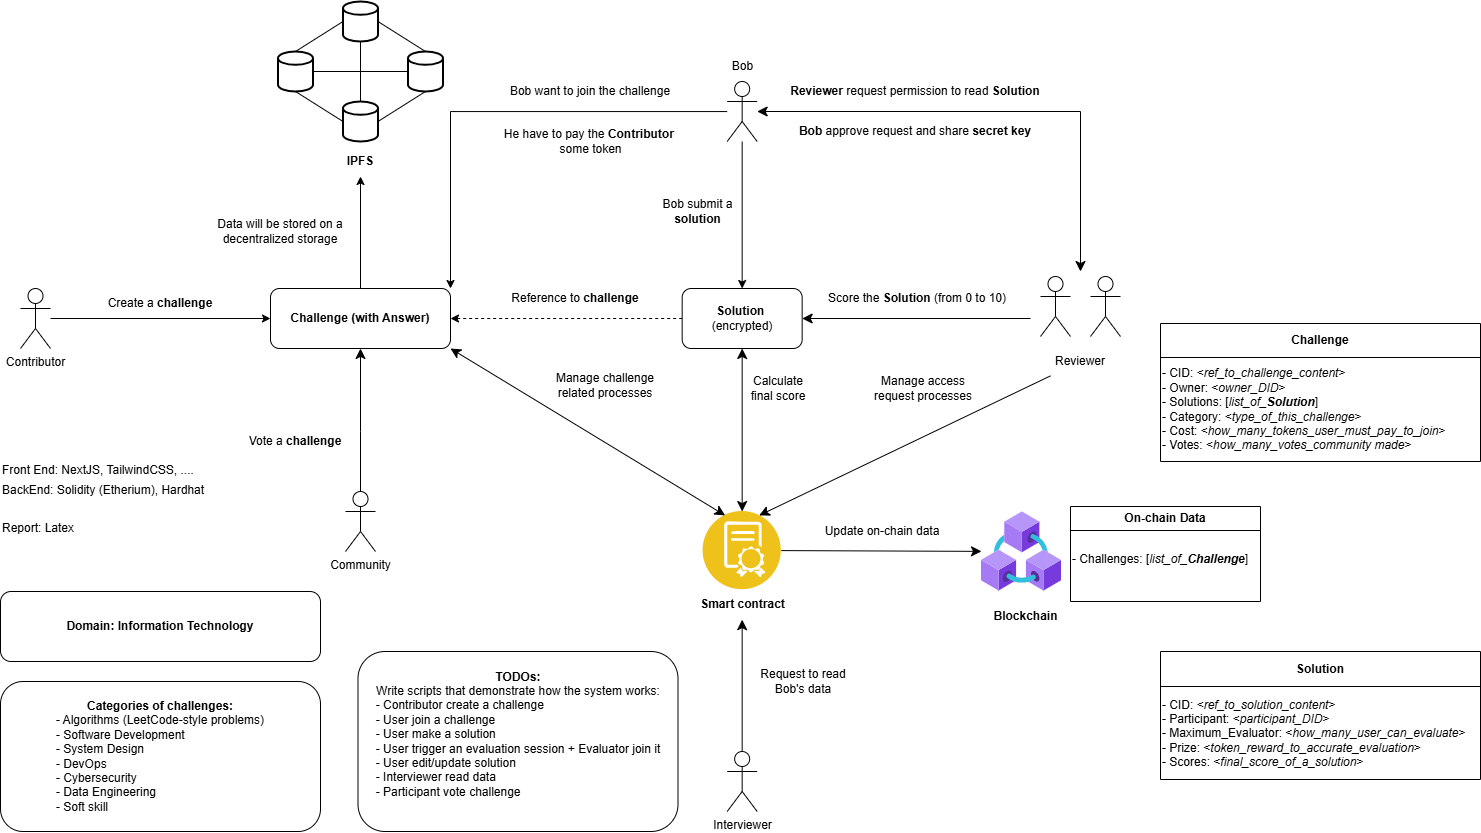
\includegraphics[width=0.97\textwidth]{prototype-v1.0.png}
  \textit{Sơ đồ hoạt động của hệ thống phiên bản 1.0}
\end{center}

\section*{Use cases}

\section*{Kế hoạch triển khai}

\section*{Tài liệu tham khảo}

\end{document}
